% Nejprve uvedeme tridu dokumentu s volbami
\documentclass[slovak,master,public,dept460,male,cpdeclaration,oneside]{diploma}
% Dalsi doplnujici baliky maker
\usepackage{subfig}		% makra pro "podobrazky" a "podtabulky"
\usepackage{tikz}		% makra pro kresleni
\usepackage{amssymb}
\usepackage{amsmath}
\usepackage{float}
\usepackage{graphicx}
\usepackage[utf8]{inputenc}
\usepackage{color}

% Zadame pozadovane vstupy pro generovani titulnich stran.
\ThesisAuthor{Veronika Uhrová}

\CzechThesisTitle{Analýza emailové komunikace}

\EnglishThesisTitle{Analysis of Email Communication}

\SubmissionDate{\now}

% Pokud nechceme nikomu dekovat makro zapoznamkujeme.
\Thanks{Moje poďakovanie patrí predovšetkým doc. Milošovi Kudělkovi, Ph.D. za odborné konzultácie a vedenie mojej diplomovej práce.}

% Zadame cestu a jmeno souboru ci nekolika souboru s digitalizovanou podobou zadani prace.
% Pokud toto makro zapoznamkujeme sazi se stranka s upozornenim.
\ThesisAssignmentImagePath{Figures/zadanie}


% Zadame soubor s digitalizovanou podobou prohlaseni autora zaverecne prace.
% Pokud toto makro zapoznamkujeme sazi se cisty text prohlaseni.
\AuthorDeclarationImageFile{Figures/prehlasenie.jpg}


\CzechAbstract{Práca študuje aktuálne metódy pre analýzu emailov a detekciu sociálnych rolí v emailových dátach. Nasleduje zoznámenie sa s emailom a jeho popularitou v súčasnosti. Taktiež práca uvádza základné teoretické pojmy a teoretický náhľad na reprezentáciu siete. Uvádzajú sa tu aj základy analýzy sociálnych sietí a detekcie komunít. Ďalej sa tu píše o frameworku pre detekciu štrukturálnych rolí a ich identifikácie. Na základe týchto poznatkov je vytvorená aplikácia pre analýzu a vizualizáciu analytických výstupov. Na záver sú uvedené prevedené experimenty týkajúce sa identifikácie sociálnych rolí v emailových dátach.}

\CzechKeywords{email, sociálna sieť, sociálna rola, vizualizácia, brokerage}

\EnglishAbstract{This paper studies current methods for analysing emails and detecting social roles in email data. This is followed by getting acquainted with the email and its popularity nowadays. Also, this thesis presents basic theoretical concepts and a theoretical overview of network representation. Here are also the basics of social networking and community detection. There is also written a framework for structural social roles detection and their identification. Based on this knowledge, an aplicaion is developed to analyze and visualize analytical outputs. Finally, experiments on the findings of the emailed data are presented.}

\EnglishKeywords{email, social network, social role, visualization, brokerage}

\AddAcronym{MUA}{Mail User Agent}
\AddAcronym{MTA}{Mail Transfer Agent}
\AddAcronym{IMAP}{Internet Message Access Protocol}
\AddAcronym{XML}{eXtensible Markup Language}
\AddAcronym{SSRM}{Structural social role mining framework}
\AddAcronym{SNA}{Social network analysis}

\DeclareCaptionType{mycapequ}[][List of equations]
\captionsetup[mycapequ]{labelformat=empty}
 

% Zacatek dokumentu
\begin{document}

% Nechame vysazet titulni strany.
\MakeTitlePages

% Pokud mame v zaverecne praci vypisy kodu, jinak odstranit.
%\lstlistoflistings

% A nasleduje text zaverecne prace.
\section{Úvod}
V stručnom úvode je popísaná motivácia, ktorá viedla k vypracovaniu tejto diplomovej práce, vízia toho, čo sa malo dosiahnuť a hrubá štruktúra vypracovaného textu.

\subsection{Motivácia}
S cieľom uľahčiť používanie emailov a prebádať podnikateľský potenciál emailov, analýza emailov dosiahla pozoruhodný pokrok v oblasti výskumu, ale aj v praxi. Emaily teda možno považovať za zmiešanú štruktúru obsahujúcu údaje o ľuďoch zo sociálnych alebo aj organizačných aspektov.

\textbf{Obsah emailu ako textové a netextové dáta} 
\newline Emaily sú písané viac stručne ako väčšina ostatných dokumentov, často obsahujú hovorové výrazy a abreviácie, ktoré sa nenachádzajú v bežných slovníkoch, preto štandartné techniky analýzy textov pri práci s emailovými dátami  nemusia byť efektívne.

Emaily tiež obsahujú bohatšie typy dát, ako napríklad URL linky, HTML tagy alebo obrázky. Niektoré štúdie jednoducho zjednodušia tieto netextové dátové vstupy v štádiu predpripravovania dát - vymažu ich a ďalej pracujú len s textovými dátami. Tieto netextové dáta však môžu byť užitočné v iných oblastiach, ako napríklad detekcia spamu. 


\textbf{Emaily reprezentujúce ľudské sociálne organizačné vzťahy} 
\newline Emailová aktivita sama o sebe reprezentuje bohaté ľudské sociálne a organizačné vzťahy, ktoré spájajú ľudí do komunít a komplexných sysémov. Porozumenie organizačných štruktúr alebo vzťahov naprieč ľudmi v organizácii môže byť veľmi užitočné aj v reálnom živote. 
Hlavné problémy, ktoré sú investigované v analýze emailov sú detekcia spamu, kategorizácia emailov, analýza kontaktov, analýza vlastností emailových sietí a vizualizácia emailov.

\subsection{Vízia}
Cieľom práce je oboznámiť čitateľa s oblasťou sociálnych sietí a špeciálne s témou analýzy emailových dát a tieto znalosti demonštrovať nad reálnymi emailovými dátami. Pre uskutočnenie tohto cieľa je potrebné naštudovať informácie z oblasti analýzy emailov, reprezentácie emailu v sieti a vizualizácie sociálnych sietí vrátanie aktuálnych metód publikovaných v článkoch. K tomu sa viaže tiež prieskum reprezentácie a konštrukcie emailu ako prvku sociálnej siete. 

Ďalej boli vybrané metódy detekcie rolí v sociálnej sieti a navrhnutá aplikácia, ktorá umožňuje analyzovať a vizualizovať analytické výsledky. V tejto aplikácii s jednoduchým a použiteľným užívateľským rozhraním budú implementované vybrané metódy analýzy a bude navrhnutá prehľadná vizualizácia vzťahov. Nakoniec bude vytvorená analýza jedného prvku siete a výsledky experimentov budú zrozumiteľne prezentované.

\subsection{Štruktúra práce}
V prvej kapitole je uvedený prieskum o aktuálnych vedeckých článkoch, ktoré sa zaoberajú analýzou emailov a reprezentácii emailu v sociálnych sieťach. Ďalej sa čitateľ zoznámi s emailom ako komunikačným prostriedkom a dozvie sa, ako sú na tom emaily s popularitou aktuálne. Potom je uvedený stručný prehľad teórie grafov a definícií určitých pojmov, ktorý je nevyhnutný k porozumeniu ďalších kapitol. V ďalšej kapitole píšem o sociálnych sieťach, ich histórii a analýze sociálnych sietí a komunitnej štruktúre sociálnych sietí. Neskôr prechádzam k popisu a reprezentácie frameworku pre detekciu štrukturálnych rolí, popisujem sociálne roly definovaná v rámci tohto frameworku a následnej v ďalšej kapitole referujem pomocou akých metód sa sociálne roly v rámci tohto frameworku identifikujú. Na základe všetkých poznatkov práce je navrhnutá aplikácia vhodná k sledovaniu sociálnych rolí v emailovej sieti.  Ešte pred záverom sú uvedené výsledky prevedených experimentov týkajúcich sa poznatkami skúmanej sociálnej siete.


\section{Súvisiace práce}

Pre odhaľovanie vzťahov medzi ľuďmi, skupina a organizáciami z emalových sietí boli aplikované mnohé techniky a modely analýzy sociálnych sietí. Mnoho štúdií použilo maily spoločnosti \textit{Enron} kvôli nedostatku dostupných veľkých súborov. 


Napríklad Diesner, Carley a Frantz v \cite{3} zkonštruovali z mailovej komunikácie spoločnosti Enron orientovaný graf zo vzťahu odosielateľ-príjemca, kde hrany boli vážené frekvenciou mailov, ktoré si medzi sebou poslali v čase. Potom aplikovali techniky analýzy sociálnych sietí. V práci popísali, ako vylepšili originálnu sadu a súčasné zistenia ich investigáciou vďaka analýze sociálnych sietí. Skúmajú dynamiku, štruktúru a vlastnosti organizačnej komunikačnej siete ako aj charakteristiky a vzory komunikačného správania zamestnancov z rôznych organizačných levelov. Zistili, že počas obdobia krízy sa komunikácia medzi zamestnancami stala viac rôznorodejšia v súvislosti so zavedenými kontaktami a formálnymi rolami. Taktiež počas obdobia kríz, predtým nekomunikujúci zamestnanci sa začali zapájať do vzájomného rozhovoru, takže interpersonálna komunikácia bola intenzívnejšia a sieť sa tým rozširovala. Tieto zistenia poskytli cenný pohľad do organizačnej krízy reálneho sveta, čo môže byť ďalej využité pre validáciu alebo tvorbu teórií a dynamických modelov organizačných kríz a tým to vedie k lepšiemu porozumeniu základných príčin organizačných kríz v organizáciách.


Xiaoyan Fu v \cite{2} prezentoval rôzne metódy pre vizualizáciu emailových sietí. Vizualizácia objavuje komunikačné vzory medzi rôznymi skupinami, zobrazuje centrálnu analýzu s dôrazom na významné uzly.
V práci zkonštruovali 2D vizualizáciu temporálnej emailovej siete, ktorá analyzuje vývoj emailových vzťahov, ktoré sa menia v priebehu času a zobrazenie prostredia pre nájdenie sociálnych kruhov odvodených od siete. Každá metóda bola vyhodnotená s rôznymi datasetmi od výskumnej orgnizácie. Taktiež rozšírili ich metódu pre vizuálnu analýzu siete emailových vírusov.

Ďalej Chapanond, Krishnamoorthy, Yener v \cite{4} použil sieťové metriky a spektrálnu analýzu k analýze či už orientovaného alebo neorientovaného grafu emailov, ktorý skonštruoval zmenou prahovej hodnoty (napr. počtom vymenených emailov medzi užívateľmi). Ich výskum je postavený na vytvorení emailového grafu a štúdiu jeho vlatností či už pomocou teórie grafov alebo technikami spektrálnej analýzy. Grafová teoretická analýza zahŕňa výpočet niekoľkých grafových metrík, ako napríklad rozdelenie podľa stupňov, priemerný pomer vzdialeností, zhlukovací koeficient alebo kompaktnosť emailového grafu. Hodnoty metrík v dátovej sade emailov spoločnosti Enron porovnali aj s inými emailovými dátami. 

Jednou z univerzálnejších prác je aj práca autorov Guanting Tang, Jian Pei, and Wo-Shun Luk \cite{1}. Je to stručný prehľad hlavných výskumných snáh o analýzu mailov a popis metód, ktoré sa pri tejto analýze používajú. Nie len čo sa týka analytických alebo implemetnačných úloh, ale aj nástrojov, ktoré nám pri analýze vedia pomôcť. Aby zdôraznili rozdiely medzi analýzou mailov a bežnou analýzou textu, organizujú prieskum do piatich ťažších úloh a to:  detekcia nevyžiadanej pošty, kategorizácia emailov, analýza kontaktov, analýza vlastností emailovej siete a vizualizácia emailov. Tieto úlohy sú vlastne začlenené do rôznych spôsobov používania emailov. Systemaicky preskúmavajú bežne používané techniky a tiež budujú diskusiu o dostupných softwarových nástrojoch.

Na rozdiel od ostatných prác, Afra Abnar, Mansoureh Takaffoli, Reihaneh Rabbany, Osmar R. Zaıane \cite{9} definovali vlastnú metodiku pre analýzu sociálnej siete a definovali \textit{Structural social role mining framework}, ktorý je navrhnutý pre identifikáciu štrukturálnych rolí, pre identifikáciu zmien v sieti a analýzu dopadu zmien na sieť. Definujú základné sociálne roly v sieti a navrhujú metodológie pre ich identifikáciu. Pre identifikáciu týchto rolí využívajú klasické prostriedky analýzy sociálnych sietí a tiež navrhujú nové metriky zahrňujúc napríklad Betweenness centrality založenú na komunitách. Z tejto práce som vychádzala pri pomenovaní rolí zo siete a implementovala techniky pre ich identifikáciu.

Ďalšou prácou, ktorou som sa inšpirovala bola práca autorov Kudělka, Horák, Zehnalová \cite{10}, ktorá prezentuje analytický nástroj, ktorý bol vytvorený pre analýzu hlbších vzťahov v emailových dátach. Tieto vzťahy zahrňujú vzťahy založené na interakcii viacerých užívateľov v tíme. Analytické metódy popísané v práci sú založené na dvoch faktoroch. Prvým faktorom je kontext, čo je skupina viacerých užívateľov v kombinácii so slovami použitými v komunikácii. Druhým faktorom je časový interval, v ktorom bola začatá komunikácia. Práca prezentuje metódy pre váženie komunikácií, užívateľov a vzťahov, ako aj metód pre hľadanie komunít asociovaných so špecifickým kontextom. 

\section{Emailová komunikácia}
\subsection{Stručná história emailu}
Za počiatky emailovej komunikácie možno považovať priližne rok 1965, kedy bola správa prenášaná medzi sálovými počítačmi pracujúcich v režime zdieľania času na univerzite \textit{Massachusetts Institute of Technology}.

Od tejto doby preša emailová komunikácia značným vývojom. Emaily, tak ako ich poznáme dnes, sú definované štandartom špecifikácie RFC2822 a sú prenášané pomocou komunikačných protokolov. 


\subsection{Štruktúra emailu}
Každý email sa skladá z dvoch častí - z tzv. hlavičky \textit{(header)} a tela emailu \textit{(body)}.

Hlavička emailu je generovaná automaticky pri vytvorení emailu a sú do nej postupne vkladané informácie zo serverov, cez ktoré správa prechádza (tzv. MTA). Pre bežných užívateľov sú z hlavičky najdôležitejšie tieto údaje: predmet správy, čas odoslania, emailová adresa odosielateľa a prijímateľa. Ostatné údaje emailoví klienti (označovaní tiež ako MUA \footnote{MUA - Mail User Agent, program, ktorý používa užívateľ na rozosielanie a prijímanie emailov (napr. Outlook), tento program komunikuje s MTA (Mail Transfer Agent), ktorý sa stará o prenos emailov v prostredí verejnej siete Internet.}) väčšinou nezobrazujú.


Pri vytváraní emailu emailovým klientom sú väčšinou do hlavičky vložené tieto záhlavia:

\begin{itemize}
\item \textbf{Date} - aktuálny čas počítača, ktorý vložil záhlavie
\item \textbf{From} - adresa odosielateľa
\item \textbf{Cc} - špecifikuje ďalších adresátov
\item \textbf{Bcc} - umožňuje rozosielanie správy medzi viacerých adresátov
\item \textbf{Priotity} - priorita emailu, interpretácia sa líši vzhľadom k MUA
\item \textbf{Reply-To} - špecifikuje adresu, na ktorú je zaslaná prípadná odpoveď
\item \textbf{Subjekt} - predmet správy daný užívateľom
\item \textbf{To} - udáva adresu príjemcu správy
\item \textbf{Message-Id} unikátny identifikátor, ktorý je priradený MTA
\end{itemize}

Telo emailu obsahuje samotné dáta určené pre adresáta. 


\subsection{Emaily v súčasnosti}
Emaily teda existujú už niečo cez 50 rokov, ich popularita je však stále veľká vďaka ich efektivite, extrémne nízkym nákladom a kompatibilite s množstvom typov zariadení. Ako jedna z najrozšírenejších typov komunikácie v dnešnej dobe, emaily sú široko rozšírené v každodennom živote. Napríklad, spolupracovníci diskutujú prácu cez emaily, priatelia zdieľajú sociálne aktivity a skúsenosti aj cez emaily alebo veľké spoločnosti distribuujú reklamy práve pomocou emailov.

Aj keď by mnohí tvrdili, že éra emailov už je dávno preč a sú stále viac nahrádzané novými sociálnymi sieťami, nové výskumy ukazujú opak. Napríklad výskum z roku 2016 od spoločnosti Bluecore \cite{13} ukazuje, že email je stále populárny aj u mladších generácií, hlavne na formálnu komunikáciu.

V tomto výskume boli spotrebitelia pýtaní, akú formu komunikácie preferujú pri komunikácii so značkami (interntovými obchodmi, na firemnú komunikáciu a celkovo formálnu komunikáciu). Prevažná časť opýtaných si vybrala email (68\%).

\begin{figure}[H]
\centering
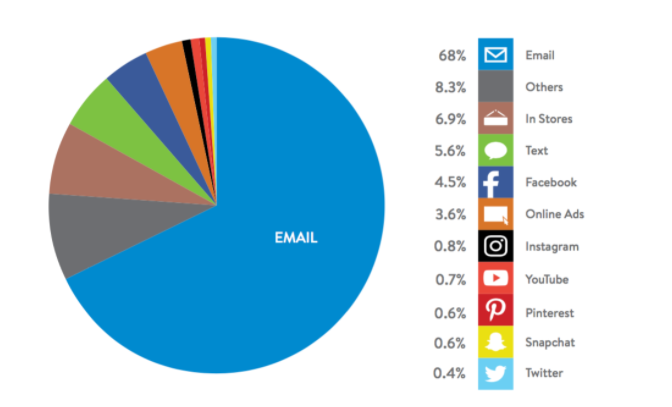
\includegraphics[width=12cm, height=7cm]{figures/emailusage}
\caption{Akú formu komunikácie preferujete na formálnu komunikáciu?}
\end{figure}


\section{Definície a klasifikácie}
V tejto kapitole popisujem všetky teoretické pojmy a metódy, ktoré v tejto práci spomínam a používam. V tejto kapitole budem používať matematické názvy podľa kontextu, v ktorom sa budem nachádzať.

\subsection{Graf}
\begin{itemize}

\item \textbf{Neorientovaný graf}

Neorientovaným grafom rozumieme usporiadanú dvojicu \textit{G = (V, E)}, kde \textit{V} je neprázdna množina \textit{vrcholov} a \textit{E} je neprázdna množina \textit{hrán} - množina (niektorých) dvojprvkových podmnožín množiny \textit{V}.

\begin{figure}[H]
\centering
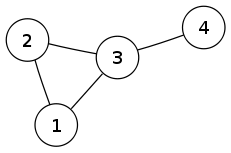
\includegraphics[width=4.5cm,height=3cm]{figures/neorientovany}
\caption{Neorientovaný graf}
\end{figure}

\item \textbf{Orientovaný graf}

Orientovaným grafom rozumieme usporiadanú dvojicu \textit{G = (V,E)}, kde V je množina \textit{vrcholov} a množina orientovaných \textit{hrán} je $E \subseteq  V \times V$. 

\begin{figure}[H]
\centering
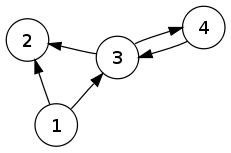
\includegraphics[width=4.5cm,height=3cm]{figures/orientovany}
\caption{Orientovaný graf}
\end{figure}

\end{itemize}
\newpage
\subsection{Súvislosť grafu}

Hovoríme, že vrchol \textit{v} je \textit{dosiahnuteľný} z vrcholu \textit{u}, ak v grafe existuje sled z vrcholu \textit{u} do vrcholu \textit{v}. Graf nazveme \textit{súvislý}, ak pre každé dva vrcholy \textit{u, v} je vrchol v dosiahnuteľný z vrcholu u. V opačnom prípade je graf \textit{nesúvislý}.

\begin{figure}[H]
\centering
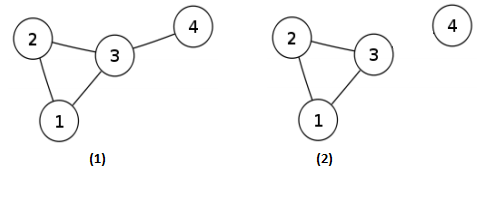
\includegraphics[width=10cm,height=4.5cm]{figures/suvisly_vs_nesuvisly}
\caption{Súvislý (1) a nesúvislý graf (2)}
\end{figure}


\subsection{Úplný graf}

Úplný graf na ${n}$ vrcholoch je neorientovaný graf, ktorý má hranu medzi každými dvoma vrcholmi. Počet jeho hrán je ${m = n ( n - 1) / 2}$.

\begin{figure}[H]
\centering
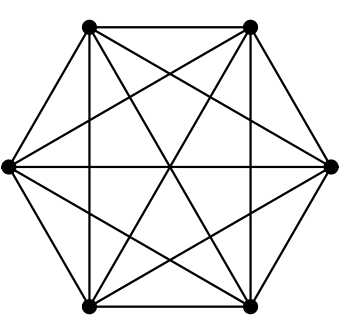
\includegraphics[width=5cm,height=4.5cm]{figures/uplnygraf}
\caption{Úplný graf}
\end{figure}


\subsection{Stupeň vrcholu}

Stupeň vrcholu je počet vrcholov spojených s týmto vrcholom hranou, inými slovami: počet jeho susedov. V orientovanom grafe sa ešte rozlišuje vstupný a výstupný stupeň vrcholu podľa toho, koľko hrán z vrcholu vychádza alebo do neho vchádza.

\subsection{Cesta}

Cesta je postupnosť vrcholov v grafe taká, že medzi každými dvoma vrcholmi cesty je hrana a vrcholy sa neopakujú. V orientovaných grafoch sa ešte rozlišuje smer cesty, pričom orientácia hrán je stále rovnaká. Dĺžka cesty je počet hrán, ktoré obsahuje.

\subsection{Uzavretá cesta}

Uzavrená cesta, kružnica v neorientovanom a cyklus v orientovanom grafe, je cesta, ktorá začína a končí v rovnakom uzle.

\subsection{Komponenta grafu}

Komponenta grafu je súvislá časť grafu a medzi vrcholmi z rôznych komponent neexistuje žiadna hrana.

\subsection{Metriky}
V tejto časti popisujem metriky, ktoré v rámci identifikácie rolí v sieti používam. Ďalšie informácie o metrikách, ich praktickom využití a ich ďalších variantách sú zhrnuté v kapitole \ref{identifikacia}.

\subsubsection{Closeness centrality (Centralita blízkosti)}
Táto centralita meria dôležitosť vrcholu grafu podľa priemernej hodnoty vzdialenosti od všetkých ostatných vrcholov v sieti. Aby dôležité vcholy mali vyššie číslo, je táto centralita počítaná ako inverzná hodnota tohto priemeru. Vrchol dôležitý podľa tejto metriky môže mať dobrý prístup k informáciám o ostaných vrcholoch alebo naopak môže ostatné vrcholz rýchlejšie ovplyvňovať.

Priemernú vzdialenosť vrcholu ${x_{i}}$ od ostatných vcholov možno formálne zapísať ako ${l_{i} = \frac{1}{n}\sum_{j}d_{ij}}$, kde \textit{n} je počet vrcholov v grafe a ${d_{ij}}$ je najkratšia cesta medzi vrcholmi  ${x_{i}}$ a  ${x_{j}}$. Centralita je potom  ${C_{i} = \frac{1}{l_{i}}}$.



\subsubsection{Betweeness centrality (Centralita medziľahlosti)}
Táto centralita sa odlišuje od ostatných uvedených. Jej hodnota pre vrchol je počet najkratších ciest medzi každými dvoma vrcholmi v grafe, na ktorých hodnotený vrchol leží. Pokiaľ medzi vrcholmi v sieti tečú nejaké informácie alebo sa posielajú správy, hodnota tejto metriky vyjadruje, aké množstvo informácií cez daný vrchol prejde. Táto centralita je tiež názorný príklad toho, že každá metrika počíta dôležitost vrcholu úplne inak. Vrchol s vysokou centralitou medziľahlosti môže mať malý stupeň a nemusí ležať blízko ostatních vrcholov, stačí, keď cez neho  prechádza veľa najkratších ciest. To môže nastať, pokiaľ vrchol je most medzi dvoma alebo viacerými komponentami v grafe, v extrémnom prípade pokiaľ je v strede grafu v tvare hviezdy (viď obrázok).

Betweeness vrcholu ${x_{i}}$ možno spočítať ako ${B_{i} = \sum_{st}^{}\frac{n^{i}_{st}}{g_{st}}}$, kde ${g_{st}}$ je počet všetkých najkratších ciest medzi vrcholmi ${x_{i}}$ a ${x_{j}}$ a ${n^{i}_{st}}$ je počet najkratších ciest, ktoré naviac vedú cez vrchol ${x_{i}}$. 

\begin{figure}[H]
\centering
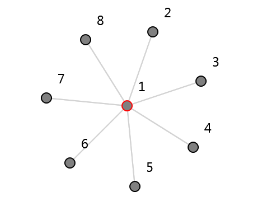
\includegraphics[width=6cm, height=5cm]{figures/graph_star}
\caption{Graf v tvare hviezdy}
\end{figure}

\subsubsection{Modularita}
Modularita je metrika, ktorá udáva rozdiel medzi počtom existujúcich hrán medzi vrcholmi rovnakého typu a počtom takých hrán v náhodne vytvorenom grafe v pomeru ku všetkým exitujúcim hranám. Vrcholy rovnakého typu sú tie, ktoré patria alebo majú patriť do rovnakej skupiny alebo triedy (komunity).

\begin{mycapequ}[!ht]
      \begin{equation*}    
{
Q = \frac{1}{2m}\sum \sum_{i,j}\begin{bmatrix}
A_{ij} - \frac{d_{i}d_{j}}{2m}
\end{bmatrix} \delta (c_{i}, c_{j})
}
   \end{equation*}
   \caption{Def: Modularita}
\end{mycapequ}


\section{Sociálna sieť}

Sociálna sieť je množina sociálnych subjektov (uzly siete, spravidla jednotlivci alebo organizácie),
ktoré sú prepojené jedným, alebo viacerými špecifickými druhmi vzájomnej závislosti, ako sú príbuzenstvo, priateľstvo, vzájomnosť, vízie, odpor, konflikt, obchod a pod.
Sociálna sieť z pohľadu teórie grafov je definovaná ako graf G(V, E), kde V je množina entít
(uzlov) a E je množnina vzťahov (hrán) medzi týmito entitami.

Entity grafu môžu byť rôzne (zákazníci, jednotlivci, webové stránky, bankové účty, creditné karty,
produkty). Nie je pravidlom, že len sociálna sieť ako ju pozná mnoho ľudí je sociálnou sieťou aj formálne. Prvky sociálnej siete môže ma napríklad aj skupina spolupracujúcich ľudí. 

\subsection{História sociálnych sietí}

Pod pojmom sociálna sieť si väčšina ľudí v dnešnej dobe predstaví služby ako \textit{Facebook, Twitter} a pod. Tento pojem ale vznikol dlho pred vznikom internetu a dnešných sociálnych sietí. Prívlastok sociálny, ktorý sa v dnešnej dobe často vynecháva, je dôsledkom pôvodu analýzy sociálnych sietí. V druhej polovici 20. storočia sa simultánne v rôznych oblastiach skúmania vzťahov a chovania objavil nový pohľad na vzťahy medzi sociálnymi jednotkami a to ako na sieť, graf. Preto prví predstavitelia analýzy sociálnych sietí boli pôvodne sociológovia alebo psychológovia (napríklad Moreno, Cartwright, Newcomb, Bavelas) a antropológovia (Barnes,Mitchell). Prvé použitie termínu "sociálna sieť" sa pripisuje Barnesovi (1954).

V 30. rokoch 20. storočia psychiater Moreno rozvíjal sociometriu, predchodcu dnešnej analýzy sociálnych sietí. Vypytoval sa ľudí na priateľské vzťahy a skúmal, ako tieto vzťahy ovplyvňujú ich chovanie. Potom vynašiel (sám to tvrdill) tzv. \textit{sociogram}, čo je diagram reprezentujúci ľudí ako body a vzťahy medzi ľuďmi ako úsečky, teda dnešnú sociálnu sieť. Tento pojem sa ale začal používať až neskôr. Pomocou neho hľadal výrazné a izolované osoby v spoločnosti.

Zhruba o 20 rokov neskôr antropológ Barnes začal skúmať, ako ovplyvnia vzťahy medzi ľuďmi nielen jednotlivcov, ale aj spoločnosť ako celok a zameral sa na štúdium skupín, komunít. Na práci Barnesa a jeho spolupracovníkov naviazala na Univerzite na Harvarde skupina vedená Harrisom Whitom. Tá začala budovať matematickú teóriu okolo dôležitejšcíh pojmov zo sociálnych vied a umožnila tieto javy matematicky vyjadriť, merať a modelovať.

V druhej polovici 20. storočia sa rozšírilo povedomie o sociálnych sieťach a metódy sa začali používať aj v ďalších oboroch ako ekonómia, biológia, doprava atd.

\subsection{Analýza sociálnych sietí}

Analýza sociálnych sietí je interdisciplinárna veda s koreňmi v sociológii, psychológii,
štatistike a teórie grafov. Analýza sociálnej siete chápe sociálnu sieť ako systém prepojenia uzlov (individuálnych aktérov) prostredníctvom hrán (ich vzťahov). Možno teda povedať, že nadväzuje na matematickú teóriu grafov a metódy sieťovej analýzy. Výsledkom analýzy môže teda byť mapa graficky znázorňujúca všetky prvky skúmaného sociálneho systému a ich vzťahy (resp. vybrané charakteristiky jednotlivých vzťahov vyjadrené vhodným spôsobom graficky). Charakteristikou môže byť napríklad vzájomná sympatia či antipatia alebo pravidelná vzájomná komunikácia alebo spolupráca.


Analýza sociálnych sietí vystupuje napríklad ako základná technika v rámci modernej sociológie,
antropológie, sociálnej lingvistiky, geografie, sociálnej psychológie, ekonómie a biológie
rovnako ako populárna téma pre výskum. 

\subsection{Komunity v sociálnych sieťach}

Sociálne siete sú riedke grafy zložené z hustých podgrafov. Tieto husté podgrafy sú nazývané
komunity. Najčastejšia definícia komunity: \textit{Komunita je zhluk uzlov, kde počet vnútorných hrán v komunite je väčší ako počet vnokajších hrán – mimo komunity}. \cite{8}

Algoritmy pre dolovanie komunít sú založené na spojoch medzi uzlami, ktoré naznačujú
spojenie dvoch entít. Napr. SCAN (Structural Clustering Algorithm for Networks) je metóda
pre detekciu komunít v súvislosti na to, ako uzly zdieľajú svojich susedov len s ohľadom na
priame spojenie. Teda ak sú dva uzly spojené a tiež zdieľajú rozumné množstvo ich susedov,
patria do rovnakej komunity.


\begin{figure}[H]
\centering
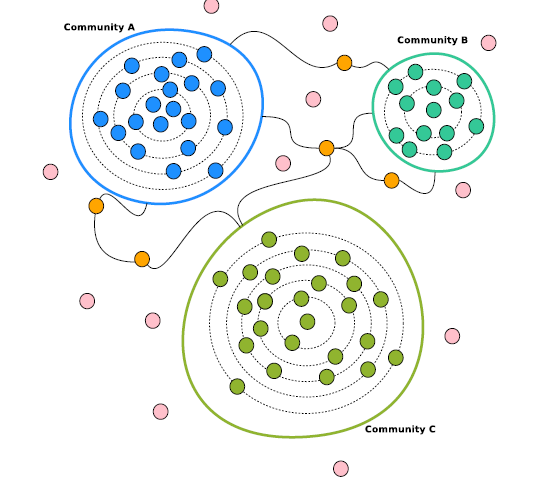
\includegraphics[width=12cm,height=10cm]{figures/comunities}
\caption{Sieť s viacerými komunitami}
\end{figure}


\subsection{Detekcia komunít}
Detekcia komunít je proces identifikácie zhlukov uzlov siete silne prepojených medzi sebou a menej silne prepojených so zvyškom siete. Detekcia komunít v grafoch má za cieľ identifikovať moduly a ich prípadnú hierarchickú organizáciu.


Problém detekcie komunít vyžaduje  rozdelenie siete do komunít husto prepojených uzlov, pričom uzly patriace do odlišných komunít sú len slabo prepojené. Presné formulácie tohto optimalizačného problému sú známe ako výpočtovo neriešiteľné. Vyhľadávanie rýchlych algoritmov pritiahlo veľký záujem vďaka zvyšujúcej sa dostupnosti rozsiahlych sieťových dátových súborov a vplyvu sietí na každodenný život. Môžeme rozlišovať niekoľko typov algoritmov detekcie komunít: \textit{rozdeľovacie} algoritmy - tie detekujú spojenie vnútri siete a postupne ich odstraňujú zo siete, \textit{algomeratívne} algoritmy - zlučujú podobné uzly a postupne komunity podľa spoločných čŕt a \textit{optimalizačné} metódy sú postavené na maximalizácii objektívnej funkcie. Kvalita rozdielov vplývajúcich z týchto metód sa často meria takzvanou modularitou. Je to hodnota v intervale od -1 do 1, ktorá meria hustotu spojov vnútri komunít v porovnaní s prepojeniami medzi komunitami. 


\subsubsection{Louvainov algoritmus pre detekciu komunít}

Veľmi obľúbeným a rýchlym algoritmom pre detekciu komunít je Louvainova metóda, ktorú navrhli Blondel, Guillaume, Lambiotte a Lefebvre \cite{12}. Je to jednoduchá metóda pre exktrakciu komunitnej štruktúry veľkých sietí. Je to heuristická metóda, ktorá je postavená na optimalizácii modularity. Je preukázané, že prekoná všetky ostatné známe metódy detekcie komunít, pokiaľ ide o čas výpočtu. Navyše kvalita detekovaných komunít je veľmi dobrá.


Výpočet algoritmu je rozdelený do dvoch fáz, ktoré sa iteratívne opakujú. Predpokladajme, že začíname s váženou sieťou s \textit{N} uzlami. Ako prvé označíme každý uzol siete inou komunitou. Takže v tomto prvotnom rozdelení je toľko komunít, ako je uzlov. Potom pre každý uzol \textit{i} uvažujeme susedov \textit{j} a vyhodnotíme prírastok modularity, ktorý by nastal, ak z sme odstránili uzol \textit{i} z jeho komunity a priradili by sme ho do komunity uzla \textit{j}. Uzol \textit{i} je potom vložený do komunity, pre ktorú je tento prírastok najvyšší, ale len ak je tento prírastok kladný. Ak nie je možný žiadny kladný prírastok, uzol \textit{i} ostáva vo svojej komunite. Tento proces je aplikovaný opätovne a sekvenčne pre všetky uzly kým sa nedosiahne žiadne zlepšenie a prvá fáza je kompletná. Prvá fáza končí, keď je dosiahnuté lokálne maximum modularity, keď žiadny uzol už nemôže zlepšiť modularitu. Je taktiež dôležité, že výstup algoritmu záleží na postupe, v ktorom sú uzly brané do úvahy. Výsledky algoritmu ale naznačujú, že usporiadanie uzlov nemá významný vplyv na získanú modularitu. Zoradenie však môže ovplyvniť výpočtový čas. Problém pri výbere objednávky preto stojí za to študovať, pretože by mohol poskytnúť dobrú heuristiku na zvýšenie výpočtového času.


Druhá fáza algoritmu spočíva vo vytvorení novej siete, ktorej uzly sú komunity nájdené počas prvej fázy algoritmu. K tomu, aby sa nová sieť vytvorila, váhy spojení medzi novými uzlami sú dané sumou váh prepojení medzi uzlami korešpondujúcih dvoch komunít. Spojenia medzi uzlami tej istej komunity vedú k slučkám v novej sieti. Keď je druhá fáza kompletná, je možné znovu aplikovať prvú fázu algoritmu na výslednú váženú sieť a proces opakovať. Pri konštrukcii sa počet komunít znižuje pri každom priechode. Proces sa opajuje, kým nie sú žiadne ďalšie zmeny a dosiahne sa maximálna modularita.


\begin{figure}[H]
\centering
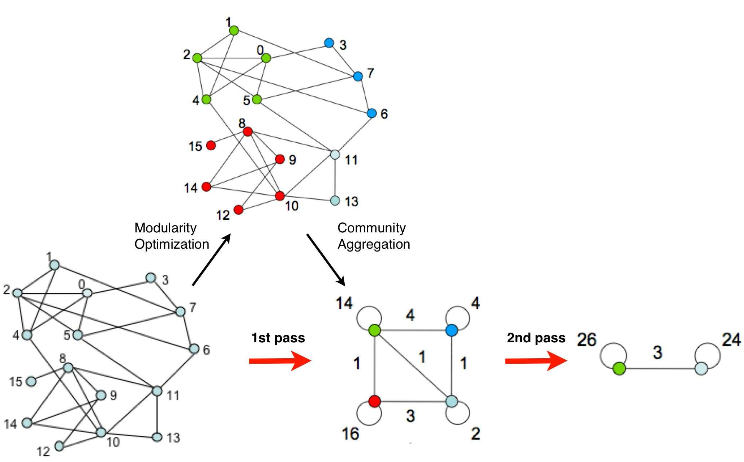
\includegraphics[width=14.5cm, height=9.5cm]{figures/louvain}
\caption{Vizualizácia krokov Louvainovho algoritmu. }
\end{figure}

Každý priechod je tvorený dvomi fázami: prvá, kde je modularita optimalizovaná tým, že umožňuje len miestne zmeny komunít a druhá, kde nájdené komunity sú agregované tak, aby bolo možné vytvoriť sieť komunít. Priechody sú opakované iteratívne kým nie je možný žiadny nárast modularity.

\newpage

\section{Metódy analýzy sociálnych sietí}

\subsection{SSRM - Framework pre detekciu štrukturálnych rolí v sociálnych sieťach}

Afra Abnar, Mansoureh Takaffoli, Reihaneh Rabbany, Osmar R. Zaıane \cite{9} definovali \textit{Structural social role mining framework}, ktorý je navrhnutý pre identifikáciu štrukturálnych rolí, pre identifikáciu zmien v sieti a analýzu dopadu zmien na sieť. Definujú základné sociálne roly v sieti(menovite Leader, Outermost, Mediator, Outsider). 

\subsubsection{Rola v kontexte SSRM}
\textit{Sociálna rola} je síce základný sociologický pojem, ale stále neexistuje žiadny konsenzus v jej definícii. Podľa SSRM je rola je považovaná za pozíciu jednotlivca v spoločnosti.
 Informácie o sociálnej sieti sú kategorizované do štrukturálnych a neštrukturálnych vlastností. Štrukturálne vlastnosti sú príbuzné ku konštrukcii grafu ako sú spojenia entít (hrany), štruktúra susedov a pozícia entity v tejto štruktúre. Ale neštrukturálne vlastnosti sú ostatné informácie, ktoré neodrážajú konštrukciu grafu ako atribúty entít a spojení. SSRM definuje rolu v sieti ako: Rola entity v sieti je to, ako sa entita správa voči ostatným a jej vplyv na atribúty a štruktúry ostatných entít.


\subsubsection{Roly definované v SSRM}
Ľudské siete sú vnútorne zložené z viacerých komunít. V sociálnej sieti s viacerými komunitami, vlastnosti uzlov kolíšu podľa toho, či je existencia komunít dostatočná alebo zanedbateľná. Z pohľadu sociálnej siete, uzol môže byť centrom celej siete, ale nie centrom v jeho komunite. SSRM sa teda zameriava na štúdium sociálnych sietí s predpokladom existencie komunít v sieti, ako jej základnej črty.

V sociálnych sieťach môžu byť komunity explicitné alebo implicitné. Explicitné komunity sú postavené nezávisle na jej členoch a sú založené na množine pravidiel. V tomto prípade, ľudia sa stanú členmi tejto komunity častejšie až po zformovaní komunity. Zamestnanci firmy alebo študenti sú príkladom dvoch explicitných komunít. Zatiaľ čo formácia implicitných komunít ťažko závisí na jej členoch a spojeniach. Tým pádom neexistuje žiadna externá podmienka na vybudovanie implicitnej komunity. Implicitné komunity sú postavené postupne ako sa ľudia spoločne stretávajú. Napríklad, skupina priateľov, v ktorej nie je žiadne pravidlo pre správanie sa jednotlivcov, je príklad implicitnej komunity. V oboch prípadoch explicitnej aj implicitnej komunity, by mali existovať aj špeciálny jednotlivci, ktorí tieto komunity manažujú a kontrolujú. Napríklad v školskej triede je to učiteľ alebo inštruktor. Pre firmu to je manažér vo vedení a pre skupinu priateľov je to zase človek, ktorého komunikačné schopnosti prinášajú ďalších členov alebo posilňujú vzťahy medzi tými stálymi. Títo dôležitý jednotlivci sú ešte viac výrazný, keď je komunita obrovská.


Podľa toho SSRM framework definuje pre jednotlivcov v sociálnej sieti určité roly podľa ich vzťahov a pozícií v komunitách až po ich interakcie s ostatnými jednotlivcami. Z perspektívy komunít, v sieti existujú jednotlivci niekoľkých typov:

\begin{itemize}
\item so žiadnym vzťahom ku nejakej komunite
\item so spojením s viacerými komunitami
\item dôležitý členovia komunity
\item bežný členovia komunity, ktorí formujú väčšinu
\item nedôležitý členovia komunity, ktorí nemajú na komunitu pozorovateľný efekt
\end{itemize} 


Na základe týchto poznatkov SSRM definuje štyri základné roly - \textbf{leader}, \textbf{mediator}, \textbf{outermost} a \textbf{outsider}.

\paragraph{Leader}
\hfill \break
Sú mimoriadni jednotlivci v zmysle centrality alebo významu v každej komunite. V reálnom svete bývajú títo členovia siete veliteľmi, riaditeľmi, manažérmi,  vládcami, prezidentami, autoritami, administrátormi atd.

\paragraph{Outermost}
\hfill \break
Je to časť menej dôležitých jednotlivcov v každej komunite, ktorých vplyv a efekt na komunitu sú nižšie ako vplyv väčšiny členov komunity. Miesta, kde sa môže outermost v sieti nachádzať sú periférie alebo hranice grafu.

\paragraph{Mediator}
\hfill \break
Sú to jednotlivci, ktorí zohrávajú dôležitú rolu v spojení komunít v medzi sebou. Fungujú ako mosty medzi odlišnými komunitami. Do tejto skupiny patria vyjednávači, sprostredkovatelia alebo aj rozbočovače v sieti. 

\paragraph{Outsider}
\hfill \break
Sú to jednotlivci, ktorí nie sú spojení so žiadnou komunitou v sieti. Buď majú takmer rovnaké prepojenie k rôznym komunitám alebo majú len veľmi slabé väzby na komunity.



\subsection{Identifikácia štrukturálnych sociálnych rolí} \label{identifikacia}
Majúc sieť s komunitami explicitne známymi alebo extrahovanými nejakým dolovacím algoritmom, následne popisujem metodológie pre identifikovanie definovaných štrukturálnych rolí.

\paragraph{Outsider}
\hfill \break
Najviac priamočiarou rolou pre identifikáciu je outsider. Je to jednotlivec, ktorý v sieti nepatrí do žiadnej komunity. Identifikácia tejto roly je tak celkom priamočiara.


\subsubsection{Leader}

Leader je v každej komunite výnimočný centrálny člen. Pre identifikovanie takýchto uzlov SSRM využíva metriku \textit{closeness centrality}.

\paragraph{Closeness centrality (Centralita blízkosti)}
\hfill \break
V súvislom grafe closeness centrality uzlu je metrika centrality v sieti, vypočítaná ako súčet dĺžok najkratsích ciest medzi uzlom a všetkými ostatnými uzlami v grafe. Čiže čím viac je uzol centrálnejší, tým bližšie je k ostatným uzlom.


\begin{mycapequ}[!ht]
      \begin{equation*}
     C_{i} = \frac{1}{l_{i}}=\frac{n}{\sum_{j}d_{ij}}
   \end{equation*}
   \caption{Def: Closeness centrality}
\end{mycapequ}


\begin{sloppypar}
Pre každý uzol sa stanoví hodnota closeness centrality. Hodnoty closeness centrality sú blízke notmálnemu rozdeleniu, v ktorom 95\% populácie dát patrí do intervalu ${\big[ \mu - 2\cdot\sigma, \mu + 2\cdot\sigma \big]}$
\end{sloppypar}

Leadri ležia na hornom chvoste distribučnej funkcie, a teda horný interval použijeme pre identifikovanie leadrov. A teda uzly, ktoré majú väčšiu hodnotu closeness centrality ako krajná hodnota tohto intervalu, sú identifikovaní ako leadri.

\subsubsection{Outermost}
Podobne ako pri role \textit{Leader} pre identifikovanie outermostov sa využíva metrika closeness centrality. Outermosti budú ležať však na spodnom chvoste distribučnej funkcie closeness centrality.

A tak teda uzlyy, ktoré majú hodnotu closeness centrality nižšiu ako ${\big[ \mu - 2\cdot\sigma \big]}$, sú outermosti.

\subsubsection{Mediator}
Rolu mediator zastávajú tí jednotlivci, ktorí spájajú viacero komunít a sú tzv. spojmy medzi komunitami. 


Pre identifikáciu mediátorov sa definujú metriky založené na metrike betweeness centrality a to:  \textit{LBetweeness - LBC} a \textit{CBetweeness - CBC} a ďalej metriky, ktoré vyjadrujú koľko rozdielnych komunít uzol spája: \textit{DSCount} a \textit{DSPair}.


\paragraph{LBeweeness}
\hfill \break
\textbf{LPath} - Pred definíciou LBetweeness je potrebné definovať LPath a to nasledovne: \textit{LPath} je množina všetkých najkratších ciest medzi lídrami dvoch rozdielnych komunít. 


\begin{mycapequ}[!ht]
   \begin{equation*}
     LPath = { l|startNode(l) \in  leaderSet(c_{i})\wedge endNode(l) \in leaderSet(c_{j}) \wedge c_{i}\neq c_{j} }
   \end{equation*}
   \caption{Def: Lpath}
\end{mycapequ}



{\setlength{\parindent}{0cm}
\begin{sloppypar}
\textbf{LBetweeness} centralita pre uzol \textit{v} - \textit{LBX(v)} je počet jedinečných LPath ktoré obsahujú \textit{v}. 


Ak pre každú cestu p  ${x \in}$ \textit{LPath} definujeme \textit{${I_l}$(p, v) = 1} ak \textit{v} leží na \textit{p}, inak \textit{${I_l}$(p, v) = 0} potom:
\end{sloppypar}
}
 
\begin{mycapequ}[!ht]
   \begin{equation*}
     LB(v) = \sum_{p \in LPath} I_{l}(p, v)
   \end{equation*}
   \caption{Def: LBetweeness}
\end{mycapequ}


\paragraph{CBetweeness}
\hfill \break
CBetweeness počíta počet najkratších ciest medzi rozdielnymi komunitami. \textit{${s_p}$} a \textit{${e_p}$} označujú štartovací a koncový uzol najkratšej cesty \textit{p} . Taktiež \textit{${c_v}$} označuje komunitu, do ktorej uzol \textit{v} patrí. Množina všetkých najkratších ciest, ktoré spájajú rozdielne komunity:  
\textit{${CPaths = \{ p | {c_s}_p \neq {c_e}_p} \}$}. Taktiež definujeme ${I_p(p, v)}$ = 1 ak \textit{v} leží na ceste \textit{p} a 0 keď neleží.


\begin{mycapequ}[!ht]
   \begin{equation*}
    CB(v) = \frac{1}{2} \sum_{p \in CPaths} I_{p}(p, v)
   \end{equation*}
   \caption{Def: CBetweeness}
\end{mycapequ}


\paragraph{Normalizovaná verzia CBetweeness}
\hfill \break
Pravdepodobnosť nájdenia viac viditeľných mediátorov vo väčších komunitách je väčšia v porovnaní s menšími komunitami. Táto situácia sa stáva, pretože vo väčších komunitách je pochopiteľne viac uzlov, čo vedie k viacerým najkratším cestám medzi nimi. Pre kompenzáciu tohoto efektu je definovaná normalizovaná verzia \textit{CBC}: 


\begin{mycapequ}[!ht]
   \begin{equation*}
    NBC(v) = \frac{1}{2} \sum_{p \in CPaths} \frac{I_{p}(p, v)}{min(|c_{s_{p}}|,|c_{e_{p}}|)}
   \end{equation*}
   \caption{Def: Normalizovaná verzia CBetweeness}
\end{mycapequ}




\begin{sloppypar}
Navrhnuté metriky \textit{CBC} a \textit{LBC} sú nevyhnutné pre identifikovanie mediátorov, ale nie sú dostatočné. Napríklad pre sieť pozostávajúcu z desiatich komunít a dvoch mediátorov \textit{${M_1}$}
a \textit{${M_2}$}, kde oba ležia na sto najkratších cestách medzi komunitami majú oba rovnaké hodnoty \textit{CBC}. Kdežto \textit{${M_1}$} spája dve rozdielne komunity, kým \textit{${M_2}$} spája všetkých 10. Pri takomto scenári \textit{${M_2}$} spája komunity viac globálne a mal by byť skôr posudzovaný ako mediátor ako \textit{${M_1}$}. A tak \textit{${SSRM}$} definuje tzv. metriku \textbf{skóre rozmanitosti}, ktorá označuje rozdielne komunity, ktoré sú prepojené cez uzol.
\end{sloppypar}


\paragraph{Skóre rozmanitosti}
\hfill \break
Táto metrika ukazuje koľko rozdielnych komunít je spojených cez špecifický uzol \textit{v}. Túto metriku definujeme v dvoch variantach:

\begin{sloppypar}
\begin{enumerate}
\item 

\textbf{DSCount} - je definovaný ako počet rozdielnych komunít, ktoré sú spojené daným uzlom. Nech \textit{${I_d}({c_i}, v)$} = 1 ak \textit{${\exists p \in CPaths: {s_p} \in {c_i} \wedge	v \in p}$}. Potom DSScount uzla \textit{v} je definované ako:


\begin{mycapequ}[!ht]
   \begin{equation*}
    DS_{count}(v) = \frac{1}{2}\sum_{c_{i}} I_{d}(c_{i},v)
   \end{equation*}
   \caption{Def: DSCount}
\end{mycapequ}


\item \textbf{DSPair} - Skóre rozmanitosti môže byť definované ako počet párov komunít, ktoré majú najmenej jednu najkratšiu cestu medzi ich členmi, ktoré prechádzajú uzlom \textit{v}. Definujeme  \textit{${I_d}({c_i},{c_j}, v)$} = 1 ak \textit{${\exists p \in CPaths: {s_p} \in {c_i} \wedge {e_p} \in {c_j} \wedge	v \in p}$}


\begin{mycapequ}[!ht]
   \begin{equation*}
   DS_{pair}(v) = \frac{1}{2}\sum_{c_{i}} \sum_{c_{j}\neq c_{i}} I_{d}(c_{i},c_{j},v)
   \end{equation*}
   \caption{Def: DSPair}
\end{mycapequ}



\end{enumerate}
\end{sloppypar}

Aj keď viac mediátorov môže mať rovnaké hodnoty jednotlivých metrík, 
môžu sa odlišovať napríklad v počte komunít, ktoré spájajú. SSRM to berie do úvahy a definuje tzv. \textit{mediacy score} ako násobok normalizovanej CBetweeness a skóra rozmanitosti:

\begin{mycapequ}[!ht]
   \begin{equation*}
 		MS(v) = NCB(v) \cdot DS_{count}(v) 
   \end{equation*}
   \caption{Def: Mediacy score}
\end{mycapequ}


\subsection{Brokerage roly}
Jednoducho povedané, \textit{brokerage} sa vyskystuje tam, keď jeden aktér siete poskytuje most medzi dvoma inými aktérmi, ktorí medzi sebou inak prepojení nie sú. Koncept \textit{brokerahe} rôl bol použitý vo veľmi veľa iných kontextoch, záleží len na jeho formalizácii. Aj keď je \textit{brokerage} tradične konceptualizovaný ako dynamický fenomén, identifikácia \textit{brokerage} rôl sa často využíva aj v oblasti statických spoločenských vzťahov. 


Jedným známym kontextom pre \textit{brokerage} je prípad obchodných vzťahov. V tomto prostredí, títo jednotlivci alebo organizácie, politické entity, ktorí boli schopní previezť tovar z jedného miesta na druhé a kontrolovať ich rozšírenie, zohrávali kľúčovú rolu v udržiavaní obchodu na regionálnej a kontinentálnej úrovni. Sprostredkovaním kontaktov medzi vzdialené tretie strany (ktoré si nemôžu vmeniť informácie inak), títo aktéri povolili uvoľnenie kritických, priestorovo lokalizovaných zdrojov naprieč rozľahlým územím, čo usnadňovalo rast zložitejších spoločností.  Kým \textit{brokerage} vo výmenných sieťach má dôležité systematické následky, jeho efekt na individuálnej úrovni bol oceňovaný viac intenzívne socilógmi (napr. v \cite{15} \cite{17} \cite{18}). 


Je zrejmé, že \textit{brokerage} sa môže vyskytnúť v mnohých nastaveniach a povaha \textit{brokerage} procesu samotného sa líši od kontextu. Vširšom zmysle tento proces spadá pod tri triedy - \textit{transfer brokerage}, v ktorom \textit{broker (ego)} vedie informácie a iné zdroje od jedného jednotlivca k druhému, ktorí nie sú priamo prepojení. Potom \textit{matchmaking brokerage}, v ktorom ego predstavuje alebo inak umožňuje spojenie jedného jednotlivca k druhému a nakoniec \textit{coordination brokerage}, v ktorom ego usmerňuje kroky ostatných a tak vyriešia svoje závislosti bez toho, aby museli byť priamo prepojení.


\textit{Brokerage} je stav alebo situácia, v ktorej účastník spája inak neprepojených účastníkov alebo zaplňuje medzery alebo diery v sieti. \cite{15} Na obrázku je \textit{broker} alebo aj \textit{spostredkovateľ} zastúpený čiernym uzlom, ktorý vyplňuje dieru v sieti alebo spojuje ostatných jednotlivcov reprezentovaných bielymi uzlami, ktoré predtým neboli navzájom prepojené priamo.

\begin{figure}[H]
\centering

\includegraphics[width=4cm, height=1cm]{figures/brokerage_example}
\caption{Príklad brokerage procesu}
\end{figure}

\textit{Broker} môže prepojiť oddelené oblasti siete sociálnymi, ekonomickými alebo politickými aspektami a preto je jediný, kto má prístup k ceneným informáciám a zdrojom z rôznych oblastí siete. \textit{Brokerage} je mechanizmus, ktorý umožňuje izolovaným či neprepojeným členom siete zdieľať informácie a zdroje a ekonomicky, politicky či spoločensky ovplyvňovať. \cite{16}

Práve kvôli spojeniu a kontrole nad jedinečnými informáciami a zdrojmi medzi neprepojenými účastníkmi siete má aktér, ktorý zohráva rolu sprostredkovateľa (\textit{broker}) v sieti väčší prístup k informáciám a zdrojom v porovnaní s tými, ktorí sprostredkovateľmi nie sú. \textit{Broker} (sprostredkovateľ) môže ťažiť z tejto kontroly nad informáciami a zdrojmi, môže sa stať silnejší v sieti a môže vykazova5 zvýšenú efektivitu vo svojej práci. \cite{16}


Detailnejšiu kategorizáciu \textit{Brokerage} rôl predstavili Gould a Fernandez \cite{15}, kde predstavili koncept \textit{brokerage} typológie. Táto typológia delí \textit{brokerage} do piatich typov na základe smeru toku informácií - tokov v sieti - a rozdeľuje aktérov do vzájomne sa vylučujúcich skupín, tried alebo organizácií.
Typy sprostredkovateľov sú \textit{liaison}, \textit{itinerant}, \textit{coordinator}, \textit{gatepeeker} a \textit{representative}.

\subsubsection{Liaison}

\textit{Liaison brokerage} je \textit{broker} spojenie medzi dvoma rozdielnymi skupinami, do ktorých on nepatrí. Na obrázku je \textit{broker} (B) spojený s dvoma skupinami (A a C), ale nie je súčasťou ani jednej tejto skupiny. 

\begin{figure}[H]
\centering
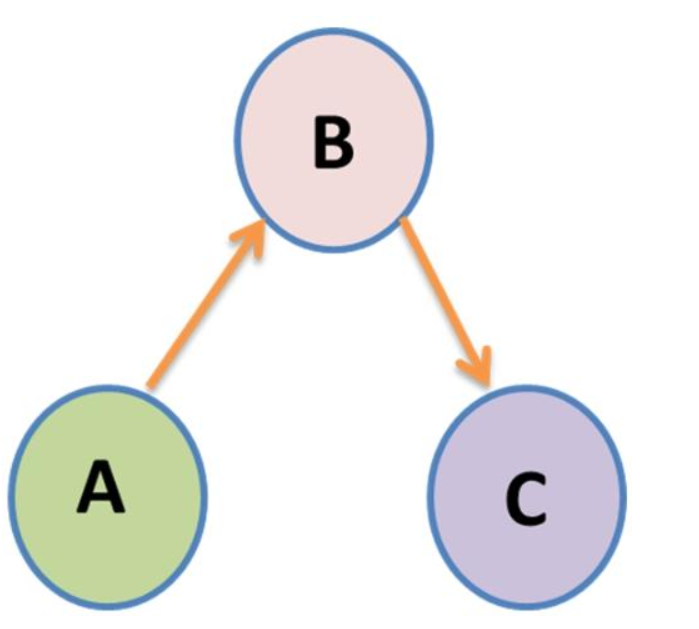
\includegraphics[width=4cm, height=4cm]{figures/liaison}
\caption{Liaison brokerage}
\end{figure}

\subsubsection{Itinerant}
Pri tomto type \textit{brokerage} roly dvaja neprepojení aktéri (A a C) patria do jednej skupiny, kým \textit{broker} (B) patrí do inej skupiny. \textit{Itinerant brokerage} je tiež nazývaný \textit{consultant brokerage}, pretože broker sa chová ako konzultant pre oboch nespojených aktérov tej istej skupiny.

\begin{figure}[H]
\centering
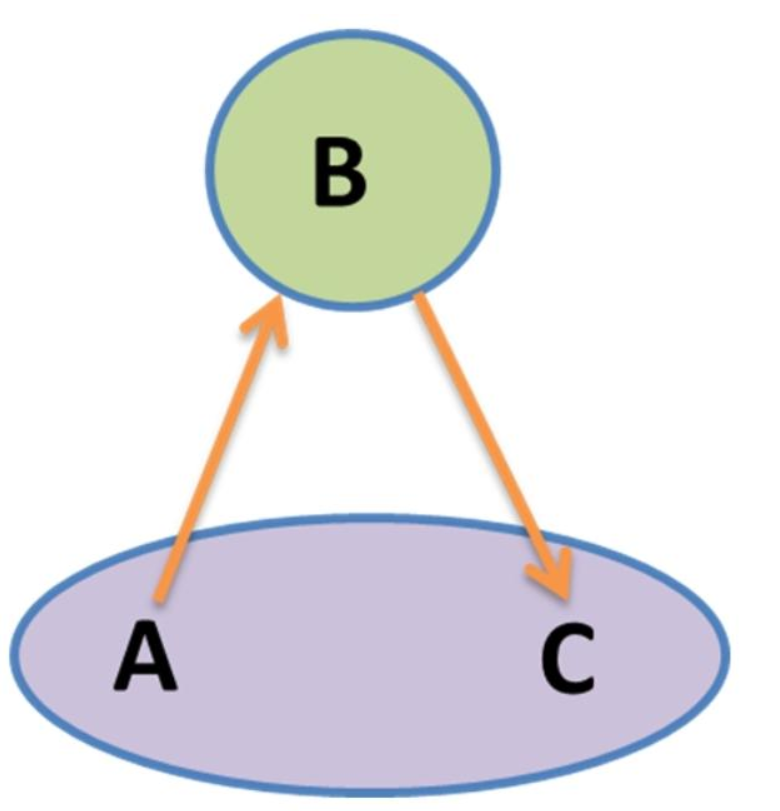
\includegraphics[width=4cm, height=4cm]{figures/itineran}
\caption{Itinerant brokerage}
\end{figure}

\subsubsection{Coordinator}
V role \textit{coordinator} všetci traja aktéri patria do rovnakej skupiny a sprostredkovanie informácií a zdrojov sa deje v rámci skupiny. 

\begin{figure}[H]
\centering
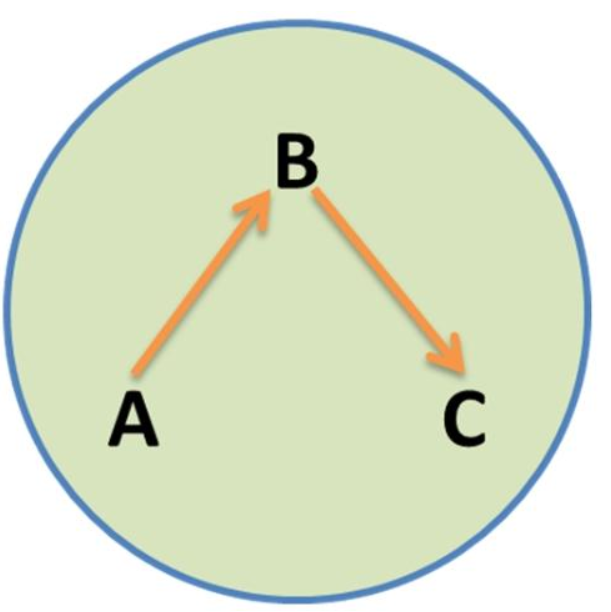
\includegraphics[width=4cm, height=4cm]{figures/coordinator}
\caption{Coordinator brokerage}
\end{figure}

\subsubsection{Gatepeeker}
V tomto type \textit{brokerage} roly \textit{broker}(B) a jeden z dvoch neprepojených aktérov (C) patria do jednej skupiny, kým iný neprepojený aktér (A) patrí do rozdielnej skupiny. \textit{Broker} tohto typu kontroluje prichádzajúce informácie a zdroje v rámci jeho skupiny a robí rozhodnutia a tom, či majú alebo nemajú neprepojení aktéri v skupine prístup k informáciám a zdrojom. 

\begin{figure}[H]
\centering
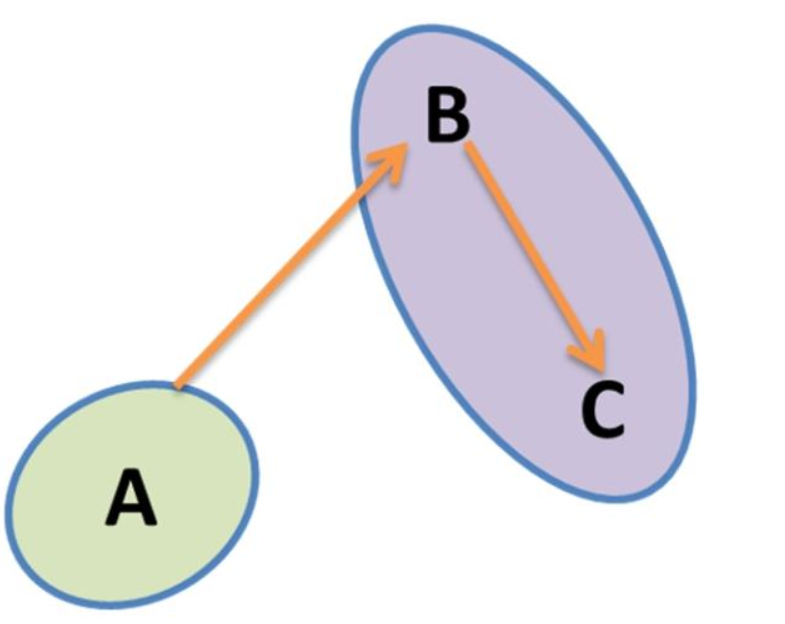
\includegraphics[width=4cm, height=4cm]{figures/gatepeeker}
\caption{Gatekeeper brokerage}
\end{figure}

\subsubsection{Representative}
\textit{Representative} rola je podobná role \textit{gatepeeker} role, \textit{broker} (B) a jeden nespojený aktér (A) patra do jednej skupiny kým ten druhý nespojený aktér (C) patrí do inej rozdielnej skupiny, ale  smer toku informácií alebo zdrojov je rozdielny. 


\begin{figure}[H]
\centering
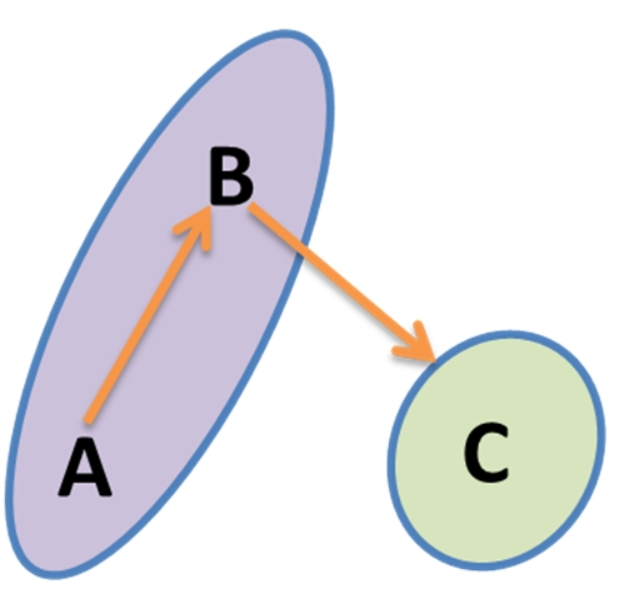
\includegraphics[width=4cm, height=4cm]{figures/representative}
\caption{Representative brokerage}
\end{figure}

\subsection{Identifikácia brokerage rolí}
Päť typov \textit{brokerage} rôl  reprezentujú unikátne sociálne roly zapúzdrujúce elementárny aspekt aktérovej štrukturálnej pozície v danej sieti. Jeden jednotlivec však môže zohrávať viac \textit{brokerage} rolí naraz. Preto Gould \& Fernandez [15] kvantifikovali celkovú participáciu jednotlivca v \textit{brokerage} rolách pomocou \textit{brokerage} skóra. Formálne definovali \textit{brokerage} v grafe reprezentujúcom asymetrickú reláciu \textit{R}: Nech \textit{a} je \textit{broker} medzi \textit{b} a \textit{c} iba ak \textit{bRa, aRc} a   ${ a\overline{R}c }$, kde \textit{bRa} indikuje, že \textit{b} je prepojené s \textit{a} reláciou \textit{R} a ${ b\overline{R}c }$
je negácia \textit{bRc}. S touto definíciou, \textit{brokerage} skóre sa vypočíta súčtom počtu koľko krát táto podmienka platí pre špecifickú kombináciu spojenia aktérov. To znamená, že ak nejaký aktér \textit{x} zohráva pozíciu \textit{coordinator} dva krát a pozíciu \textit{representative} tri krát, tak aktér bude mať skóre pre pozíciu \textit{coordinator} = 2, pre pozíciu  \textit{representative} = 3 a jeho celkové \textit{brokerage} skóre bude 5.


\section{Aplikácia}
Táto kapitola obsahuje všetky podrobnosti o vývoji aplikácie, návrhu a ďalej špecifikáciách požiadavkov. Sú tu uvedené informácie o implementácii, návrhu, návrhových vzoroch, ale aj  konštrukcii siete, predpríprave dát. Táto časť taktiež obsahuje diagramy najdôležitejších tried aplikácie alebo diagramy prípadov použitia. 


\subsection{Špecifikácia}
Aplikácia slúži ako užívateľské rozhranie na anlýzu emailovej komunikácie a vizualizáciu analyytických výstupov. Aplikácia umožňuje exportovať dáta z emailovej schránky alebo importovať vlastný XML súbor s emailovými dátami a ďalej s týmito dátami pracovať a zobrazovať sieť emailovej komunikácie. Umožňuje vytvorenie ego-siete alebo detekovať vo vytvorenej siete komunity. Najdôležitejšou časťou aplikácie je detekcia štrukturálnch rolí v sieti, čiže detekcia dôležitých a nedôležitých členov emailovej komunikácie. 


\subsubsection{Funkčné požiadavky}
\begin{itemize}
\item Export dát z emailovej schránky
\item Import vlastného XML súboru s emailovými dátami
\item Zobrazenie informácii o emailovej sieti
\item Vizualizácia emailovej siete
\item Vytvorenie ego-siete
\item Detekcia komunít
\item Detekcia štrukturálnych rolí v sieti
\item Výber časového rozmedzia emailových konverzácií
\end{itemize}


\begin{figure}[H]
\centering
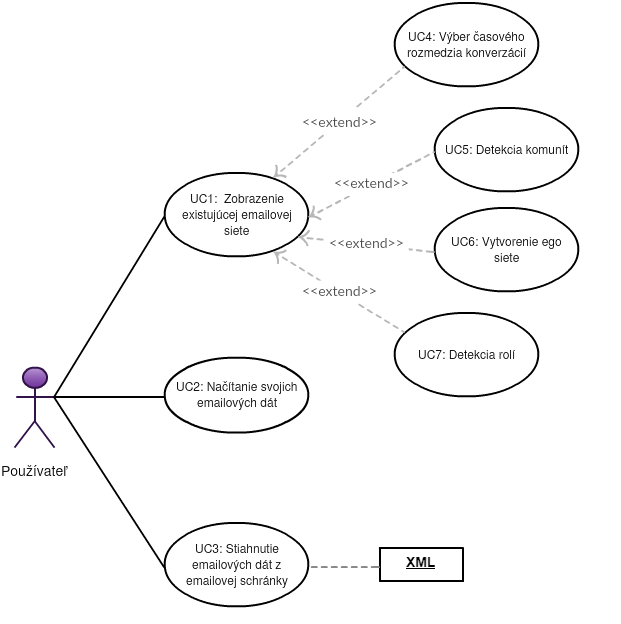
\includegraphics[width=12cm, height=12cm]{figures/diagram_usecase}
\caption{UseCase Diagram}
\end{figure}


\subsection{Návrh}
Aplikácia je vytvorená ako .NET aplikácia (veria .NET Frameworku 4.6). Je vytvorená ako trojvrstvová, pre uloženie dát sa používa SQL databáza. Najnižšia vrstva aplikácie slúži na získavanie dát z databázy, pre prepojenie s databázou a posielanie dát z aplikácie do databázy používam Entity Framework a používam tu návrhový vzor Repository. Od tejto časti je oddelená časť s business logikou a na najvyššej časti, ktorá slúži len na zobrazenie dát a komunikáciu s užívateľom, používam známy prístup Model-View-Controller.


\begin{figure}[H]
\centering
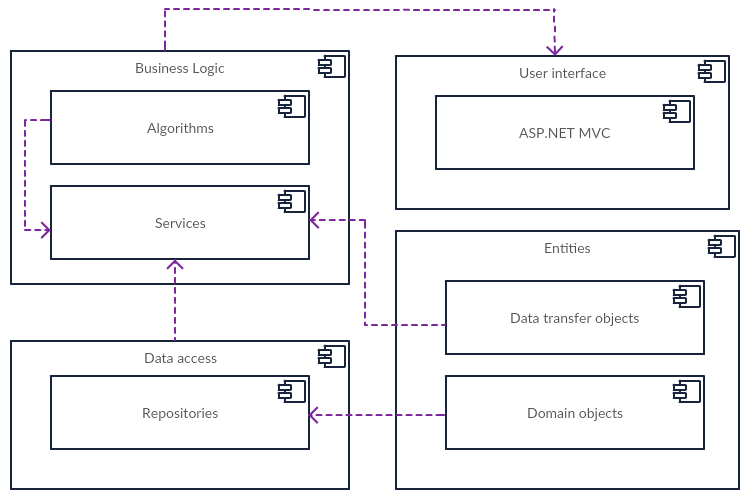
\includegraphics[width=15cm, height=9cm]{figures/diagram_komponent}
\caption{Diagram komponent znázorňujúci jednotlivé komponenty architektúry aplikácie}
\end{figure}

\subsubsection{Návrhové vzory}

\indent
\indent \textbf{Repository}
Návrhový vzor Repository je základným kameňom doménou riadeného návrhu. Model aplikácie teda nemá poňatie o tom, akým spôsobom je perzistovaný. O to sa stará práve Repository. Naviac práve vďaka tomu, že sa o persistenciu stará cudzí objekt, stačí poznať len jeho rozhranie a v prípad potreby ho ľahko nahradiť iným. \cite{11}

\begin{figure}[H]
\centering
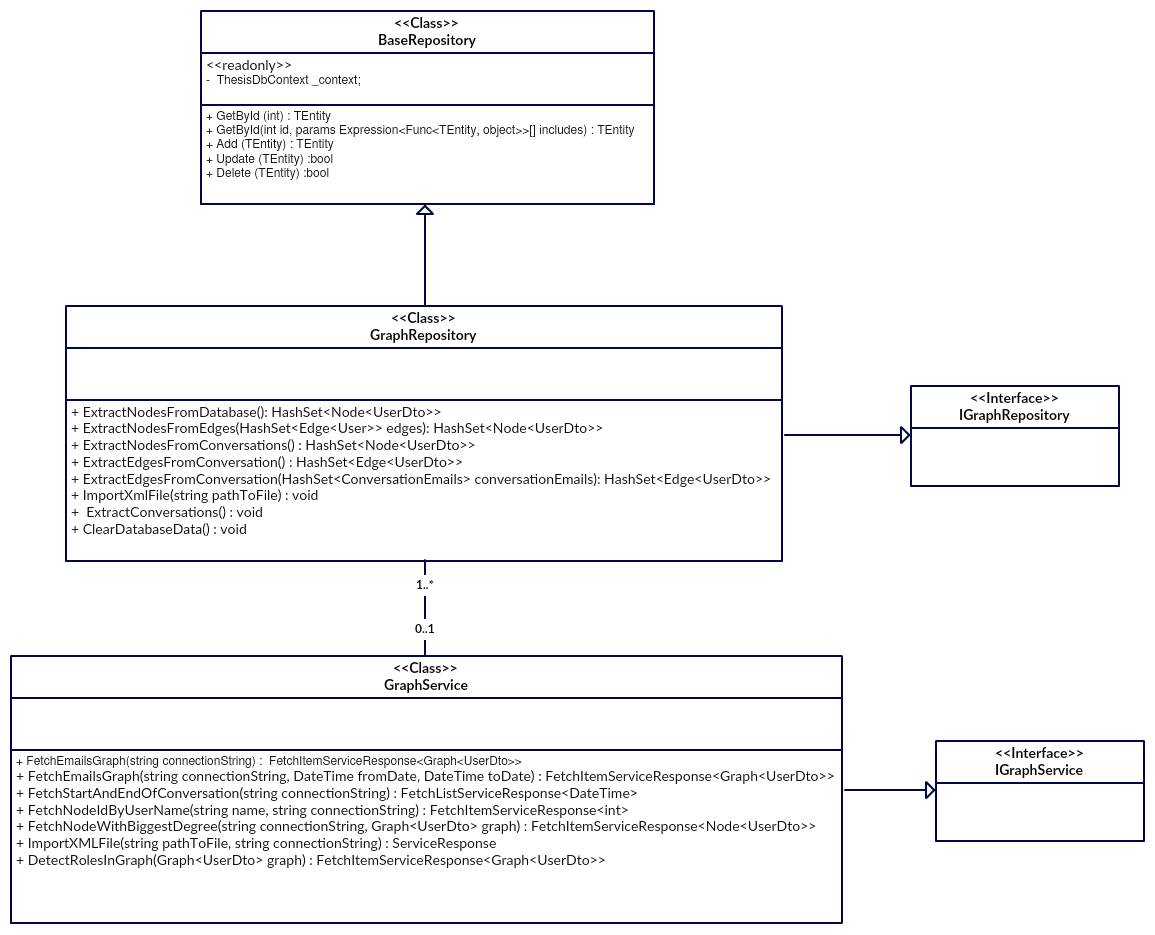
\includegraphics[width=13cm, height=14cm]{figures/diagram_class}
\caption{Triedny diagram - Repository pattern}
\end{figure}



\textbf{Model-View-Controller}
V aplikácii je použitý tradičný vzor Model View Controller (MVC). Je to jeden z najpoužívanejších a najobecnejších architektonických vzorov. 

MVC rozdeľuje program do troch hlavných častí:
\begin{itemize}
\item \textbf{Model} - dáta a súvisiace operácie 
\item \textbf{View} - prezentácia dát (užívateľslé rozhranie), obsahuje priamy odkaz na model, aby mohol jeho dáta prezentovať vonkajšiemu svetu
\item \textbf{Controller} - riadi tok udalostí v programe, konkrétne v tejto aplikácii kontrolery obsahujú len volanie metód z inej vrstvy aplikácie
\end{itemize}

\begin{figure}[H]
\centering
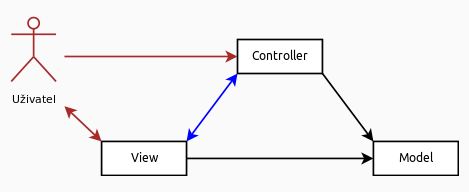
\includegraphics[width=9.5cm, height=5cm]{figures/MVC}
\caption{Model-View-Controller}
\end{figure}


\subsection{Dôležité rozhodnutia}
Pri navrhovaní aplikácie bolo potrebné urobiť niekoľko dôležitých rozhodnutí.

\subsubsection{Dostupnosť dát}
Pôvodne sa zvažovalo použitie aplikácie a analýzy dát nad verejne dostupnou anonymizovanou emailovou sadou. Emailových dát je ale veľmi málo a chcela som, aby sa výsledky práce dali overiť nie len inými analytickými nástrojmi, ale aj empiricky. Takže som využila to, že pracujem a moja emailová schránka teda nie je chudobná na maily. Navyše mi radi pomohli aj moji kolegovia a poskytli mi svoje emailové dáta. Takto som zozbierala reálne emailové dáta štyroch ľudí, o ktorých je známe ich postavenie v týme alebo aj dátum nástupu do práce. Takže výsledky daných algoritmov som vedela porovnať s reálnou situáciou v kolektíve.

\subsubsection{Webová vs. desktopová aplikácia}
Bolo nutné sa rozhodnúť, či vyvíjať aplikáciu ako webovú alebo desktopovú. Ako platforma bola zvolená Microsoft .Net a programovací jazyk C\#. Jednou z variant bola desktopová aplikácia vyvíjaná vo Windows Forms. WinForms je osvedčná technológia, je vyladená, v základe obsahuje veľké množstvo grafických prvkov. Toto sú výhody rozšírenej a dlho používanej technológii. Nevýhoda je ale práve zastaralosť a ťažkopádnosť v kreslení a spravovaní grafického rozhrania. Keďže ale doba ide dopredu a web a webové aplikácie sú stále viac používanejšie a v súčasnosti existuje mnoho grafických knižníc pre vizualizáciu grafického rozhrania, rozhodla som sa aplikáciu vyvíjať ako webovú.


\subsection{Použité knižnice}


\textbf{vis.js}


\noindent Vis.js je dynamická vizualizačná knižnica. Knižnica je navrhnutá tak, aby bola ľahko ovládateľná a aby mohla spracovať veľké množstvo dynamických dát a umožňovala manipuláciu s dátami a interakciu s nimi. Knižnica sa skladá z častí \textit{DataSet, Timeline, Network, Graph2d} a \textit{Graph3d}.
Pre moju aplikáciu som používala len časť \textit{Network}.

\begin{figure}[H]
\centering
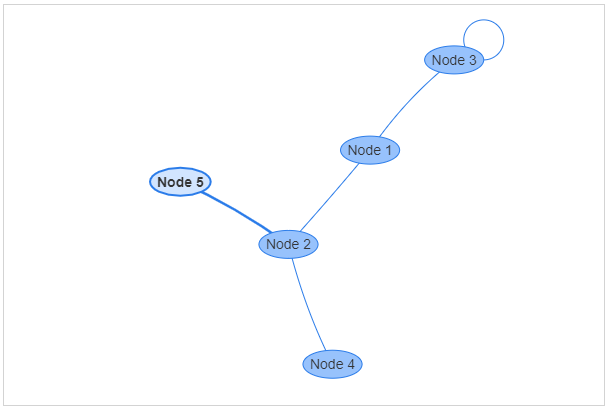
\includegraphics[width=9.5cm, height=6.5cm]{figures/vis_basic_usage}
\caption{Jednoduchá sieť vytvorená s použitím knižnice vis.js}
\end{figure}


\begin{figure}[H]
\centering
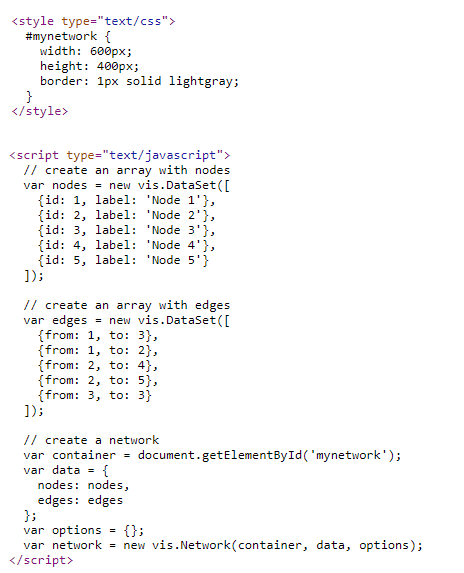
\includegraphics[width=9.5cm, height=12cm]{figures/vis_basiccode}
\caption{Príklad použitia knižnice vis.js}
\end{figure}




\subsection{Import dát}
Do aplikácie je možné nahrať XML súbor, ktorý je spracovaný uloženou SQL procedúrou, ktorá rozparsuje emailové dáta na jednodlivé entity - \textit{User, EmailMessage, UserEmail} a \textit{Conversation} a uloží ich do SQL databázy.


\begin{figure}[H]
\centering
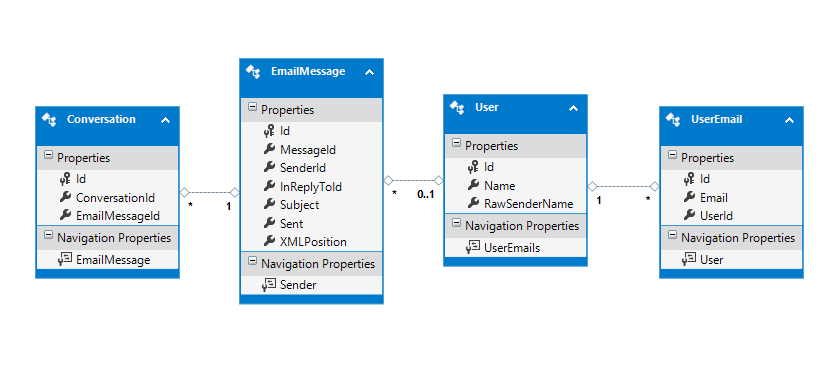
\includegraphics[width=16cm, height=8cm]{figures/domain_model}
\caption{Doménový model}
\end{figure}

\subsection{Implementácia}
Aplikácia je napísaná v jazyku C\#, grafické rozhranie je naimplementované pomocou návrhového vzoru Model View Controller a graf bol vizualizovaný pomocou knižnice vis.js. Aplikácia bola vyvíjaná vo Visual Studiu 2017.

\subsubsection{Konštrukcia siete}
Rozdiel medzi prísupom rôznych štúdií a mojím prístupom pri konšrukcii grafu z emailového datasetu je v konštrukcii komunikačnej siete. Ako základnú stavebnú jednotku siete som si zvolila \textbf{konverzáciu}. Inšpirovala som sa prácou autorov Kudělka, Horák, Zehnaloová \cite{10}. Konverzácia je teda súbor emailov, ktorá začína jediným emailom, obsahuje najmenej 2 emaily a dvoch rôznych odosielateľov. Vrcholom siete (grafu) sa teda stane užívateľ, ktorý bol ako odosielateľ aspoň v jednej takejto konverzácii. Hrana medzi užívateľmi je zostrojená medzi užívateľmi, ktorí boli spolu v jednej konverzácii ako odosielatelia. Pre konverzáciu ešte ukladám čas jej začiatku, užívateľ si následne v aplikácii môže zvoliť časový rozsah konverzácií.

\subsubsection{Triedy pre graf, vrcholy a hrany}
Pre uloženie siete v pamäti slúži generická trieda \texttt{Graph<T>}. Vrcholy a hrany drží ako \texttt{Dictionary<int, HashSet<Node<T>{}>{}>}, čiže ako mapu vrcholov s ich susednými vrcholmi. Pre uloženie vrcholov a hrán grafu slúžia zoznamy hrán a vrcholov uložené ako \texttt{HashSet<Node<T> >} a \texttt{HashSet<Edge<T>{}>}. Trieda je generická preto, aby bolo možné vytvoriť graf pre rôzne entity. Triedy reprezentujúce vrcholy a hrany sú tiež generické a predstavujú ich \texttt{Node<T>} a \texttt{Edge<T>}. Pre identifikáciu komunity, bola vztvorená trieda \texttt{Comunity<T>}.



\section{Experimenty}

\subsection{Príprava dát}


\subsection{Import dát}


\subsection{Vizualizácia}


\subsection{Detekcia komunít}
\subsubsection{Zmeny komunít v čase}

\subsection{Ego sieť}
\subsubsection{Zmeny siete v závislosti nad voľbou ega}


\subsection{Analýza rolí}
\subsubsection{SSRM}
\subsubsection{Brokerage}



	
	


\section{Záver}
\subsection{Možnosti rozšírenia a zdokonalenia práce}



\newpage
\begin{thebibliography}{99}
	\bibitem{1} Guanting Tang, Jian Pei, and Wo-Shun Luk
		\newline
		\textit{Email Mining: Tasks, CommonTechniques, and Tools}
	 
	\bibitem{2} Xiaoyan Fu 
		\newline
		\textit{Visualization and Analysis of Email Networks}
	
	\bibitem{3} J. Diesner, T. L. Frantz, and K. M. Carley
		\newline
		\textit{Communication networks
from the enron email corpus it’s always about the people. Enron is no different}

	\bibitem{4} A. Chapanond, M. S. Krishnamoorthy, and B. Yener 
		\newline
	 	\textit{Graph Theoretic and Spectral Analysis of Enron Email Data }
	
	\bibitem{5} TeamNETData
		\newline
		\texttt{http://inflex.cz:8075/TeamNETdata/}
	
	\bibitem{6} N. Crossley, E. Bellotti, G. Edwards, M. G. Everett, J. Koskinen, M. Tranmer 
		\newline
	 	\textit{Social network analysis for Ego-Nets}	
	
	\bibitem{7} Petr Kovář
		\newline
		\textit{Úvod do Teorie grafů} - skripta VŠB 
	
	\bibitem{8} M.E.J. Newman
		\newline
		\textit{The structure and function of complex networks}
	
	\bibitem{9} Afra Abnar, Mansoureh Takaffoli, Reihaneh Rabbany, Osmar R. Zaıane 
		\newline
		\textit{SSRM: Structural Social Role Miningfor Dynamic Social Networks}
	
	\bibitem{10} Zehnalová, Horák, Kudělka
		\newline
		\textit{Email Conversation Network Analysis: Work Groups and Teams in Organizations}
	
	\bibitem{11} Repository pattern 
		\newline
		\texttt{https://www.rarous.net/weblog/271-active-record-vs-repository-pattern.aspx}
	
	\bibitem{12} Vincent D. Blondel, Jean-Loup Guillaume1, RenaudLambiotte and Etienne Lefebvre
		\newline
		\textit{Fast unfolding of communities in large networks}
	
	\bibitem{13} Do Millennial and Gen Z Consumers Still Use Email? 
		\newline
		\texttt{https://www.bluecore.com/blog/do-millennials-use-email/}
		
	\bibitem{14} vis.js
		\newline
		\texttt{http://visjs.org/}
		
	\bibitem{15} Roger V. Gould and Roberto M. Fernandez
		\newline
		\textit{Structures of Mediation: A Formal Approach to Brokerage in
	 Transaction Networks}
	 
	\bibitem{16} Stovel, K. and Shaw, L.
		\newline
		\textit{Brokerage. Annual Review of Sociology}
		
	\bibitem{17} Marsden,P.V.
		\newline
		\textit{Brokerage behavior in restricted exchange networks}
		
	\bibitem{18} Burt,R.S.
		\newline
		\textit{Structural Holes: The Social Structure of Competition}	

	\bibitem{19}  Emma S. Spiroa,Ryan M. Actonb,Carter T .Butts
		\newline						
		\textit{Extended structures of mediation: Re-examining brokerage in dynamic networks}
		
	\bibitem{20} Anil Kumar Chaudhary and Laura A. Warner
		\newline						
		\textit{Introduction to Social Network Research: Brokerage Typology}	
\end{thebibliography}


\end{document}
